\chapter{Implementasi dan Pengujian}
\label{chap:implementasiPengujian}

Bab ini terdiri atas dua bagian, yaitu Implementasi Perangkat Lunak dan Pengujian Perangkat Lunak. Bagian implementasi berisi penjelasan lingkungkan pengembangan perangkat lunak dan hasil implementasi. Sedangkan bagian pengujian berisi hasil pengujian fungsional dan eksperimental terhadap perangkat lunak yang telah dibangun.

\section{Implementasi}
\label{sec:implementasi}

\subsection{Lingkungan Implementasi}
		\label{sec:lingkungan_implementasi}
			Lingkungan implemementasi yang digunakan adalah Heroku. Heroku merupakan \textit{cloud platform} yang menyediakan fitur yang dapat membantu pengguna untuk dapat memiliki alamat domain. Semua aplikasi Heroku dijalankan dalam koleksi kontainer Linux ringan yang disebut dynos. Spesifikasi Heroku yang digunakan oleh IFStudentPortal akan dijelaskan pada Tabel \ref{tab:dynotype}
\begin{table}[H]
	\centering
		\caption{Spesifikasi Heroku}
			\begin{tabular}{ |p{1.5cm}|p{1.5cm}|p{2cm}|p{1.5cm}|p{1.5cm}|p{1.5cm}|p{1.5cm}|}
			\hline
			Dyno Type & Sleeps & Professional Features & Memory (RAM) & CPU Share & Dedicated & Compute \\ \hline
			free & yes & no & 512 MB & 1x & no & 1x-4x \\ \hline
			\end{tabular}
		\label{tab:dynotype}
\end{table}
			Dari tabel diatas akan dijelaskan detail dari masing-masing kolom, yaitu:
			\begin{enumerate}
				\item \textbf{Dyno Type}, Heroku menyediakan sejumlah \textit{dyno type} yang berbeda masing-masing dengan satu set properti unik dan karakteristik kinerja.
				\item \textbf{Sleeps}, jika aplikasi memiliki \textit{web dyno}, dan \textit{web dyno} tidak menerima \textit{traffic} dalam periode 30 menit, \textit{web dyno} akan tidur. Selain \textit{web dyno} yang sedang tidur, \textit{worker dyno} (jika ada) juga akan tidur. Jika \textit{web dyno} tidur menerima \textit{web traffic}, maka akan menjadi aktif kembali setelah penundaan singkat. Jika aplikasi memiliki \textit{worker dyno} yang ditingkatkan sebelum tidur, maka akan ditingkatkan lagi juga.  
				\item \textbf{Professional Features}, fitur profesional seperti \textit{horizontal scalability, application metrics, dan preboot}
				\item \textbf{Memory (RAM)}, RAM yang digunakan adalah sebesar 512 MB.
				\item \textbf{CPU Share}, menentukan alokasi daya pemprosesan yang dialokasikan ke \textit{Virtual Machine} dalam layanan \textit{Cloud}.
				\item \textbf{Compute}, Heroku \textit{compute unit} hanya \textit{Amazon compute unit} (karena Heroku berjalan diatas AWS). Satu unit komputasi pada AWS didefinisikan sebagai kekuatan komputer dari 1.0-1.2Ghz dari \textit{CPU server 2007}.
			\end{enumerate}
				
\subsection{Hasil Implementasi}
		Hasil implementasi berupa aplikasi berbasis web yang dikembangkan untuk menyesuaikan dengan StudentPortal Baru dan Kurikulum 2018. Aplikasi dapat diakses dengan URL \url{https://ifstudentportalskripsi.herokuapp.com}. Aplikasi Informatika Student Portal terdiri dari lima halaman antara lain:
		\begin{enumerate}
			\item\textbf{Halaman \textit{Login}}\\
				Halaman \textit{login} digunakan pengguna untuk masuk ke dalam aplikasi. Pada halaman ini, pengguna dapat melakukan \textit{login} dengan mengisi \textit{email} pada kolom \textit{email} dan \textit{password} pada kolom \textit{password} kemudian mengklik tombol login. Tangkapan layar dari halaman \textit{login} dapat dilihat pada Gambar \ref{fig:5_halaman_login}.
					\begin{figure}[H]
						\centering
						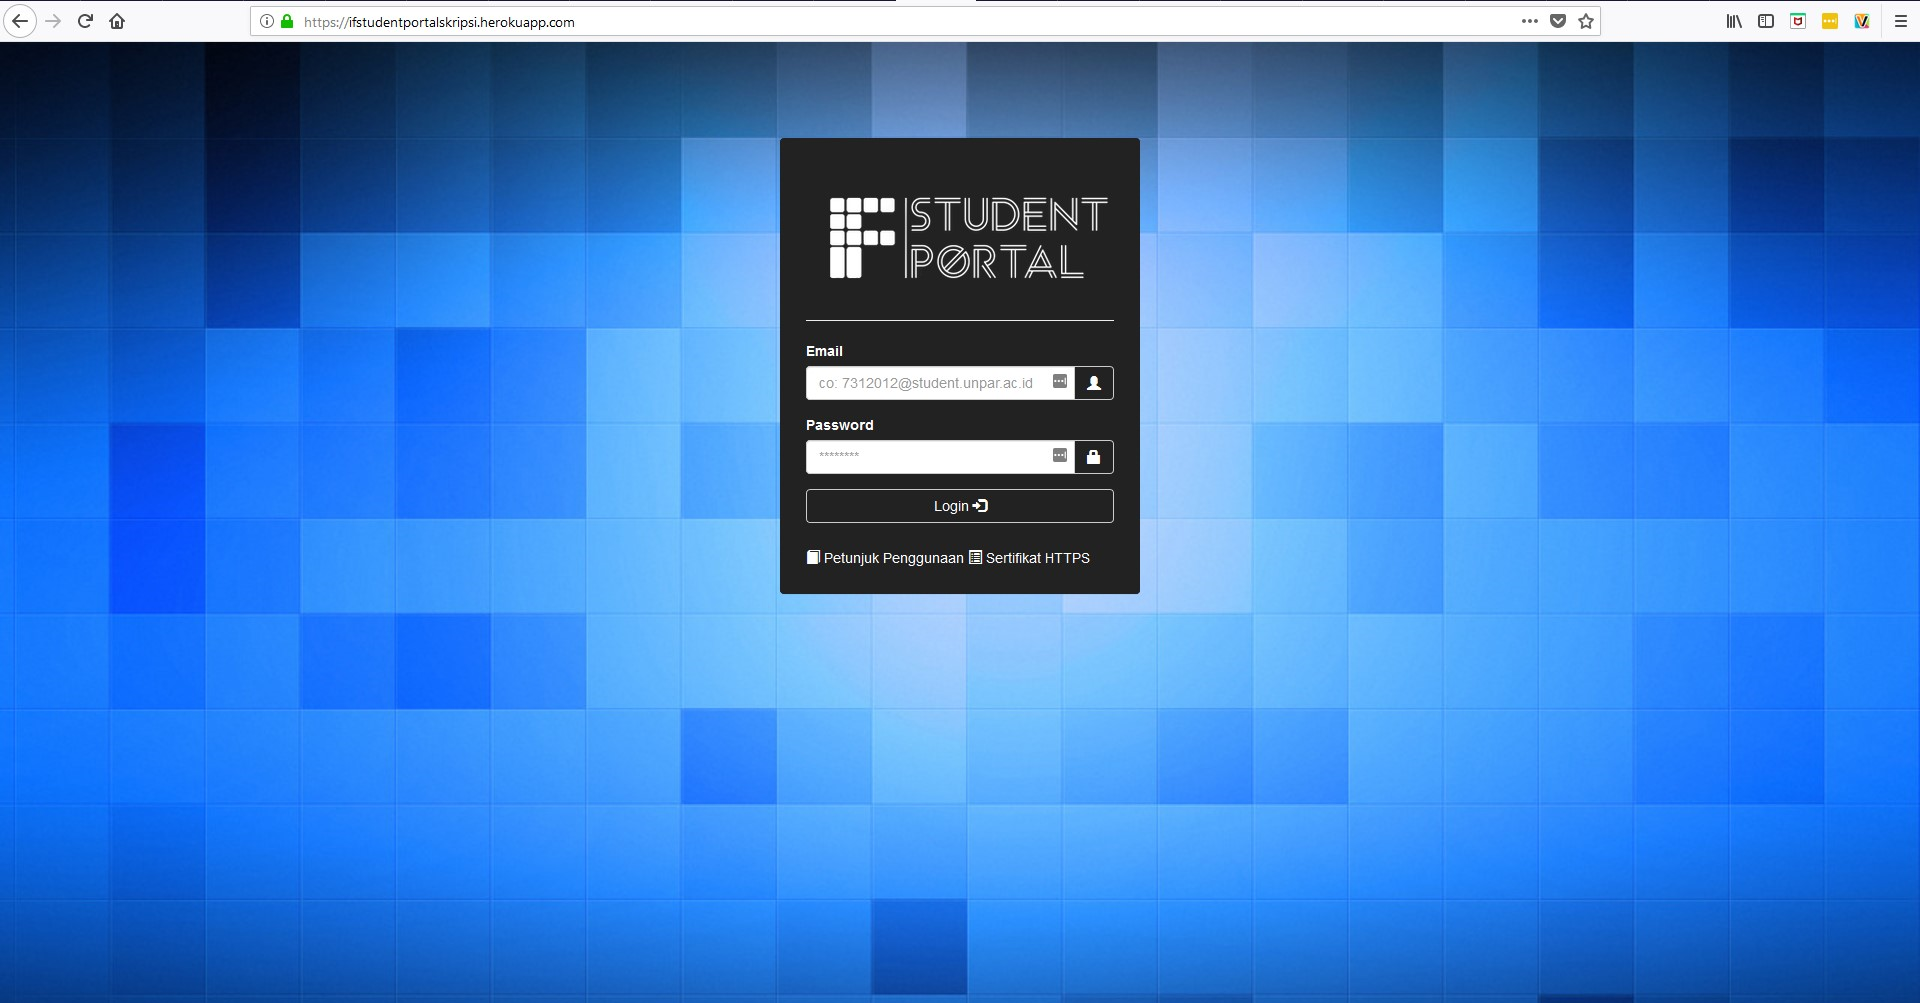
\includegraphics[scale=0.34]{Gambar/halaman_login}
						\caption{Halaman \textit{Login}} 
						\label{fig:5_halaman_login}
					\end{figure}
					
				\item\textbf{Halaman \textit{Home}}\\
				Halaman utama merupakan halaman yang pertama kali dituju setelah melakukan \textit{login}. Halaman utama menampilkan identitas pengguna dan \textit{link} menuju kode sumber aplikasi Informatika Student Portal. Tangkapan layar dari halaman utama dapat dilihat pada Gambar \ref{fig:5_halaman_utama}.
					\begin{figure}[H]
						\centering
						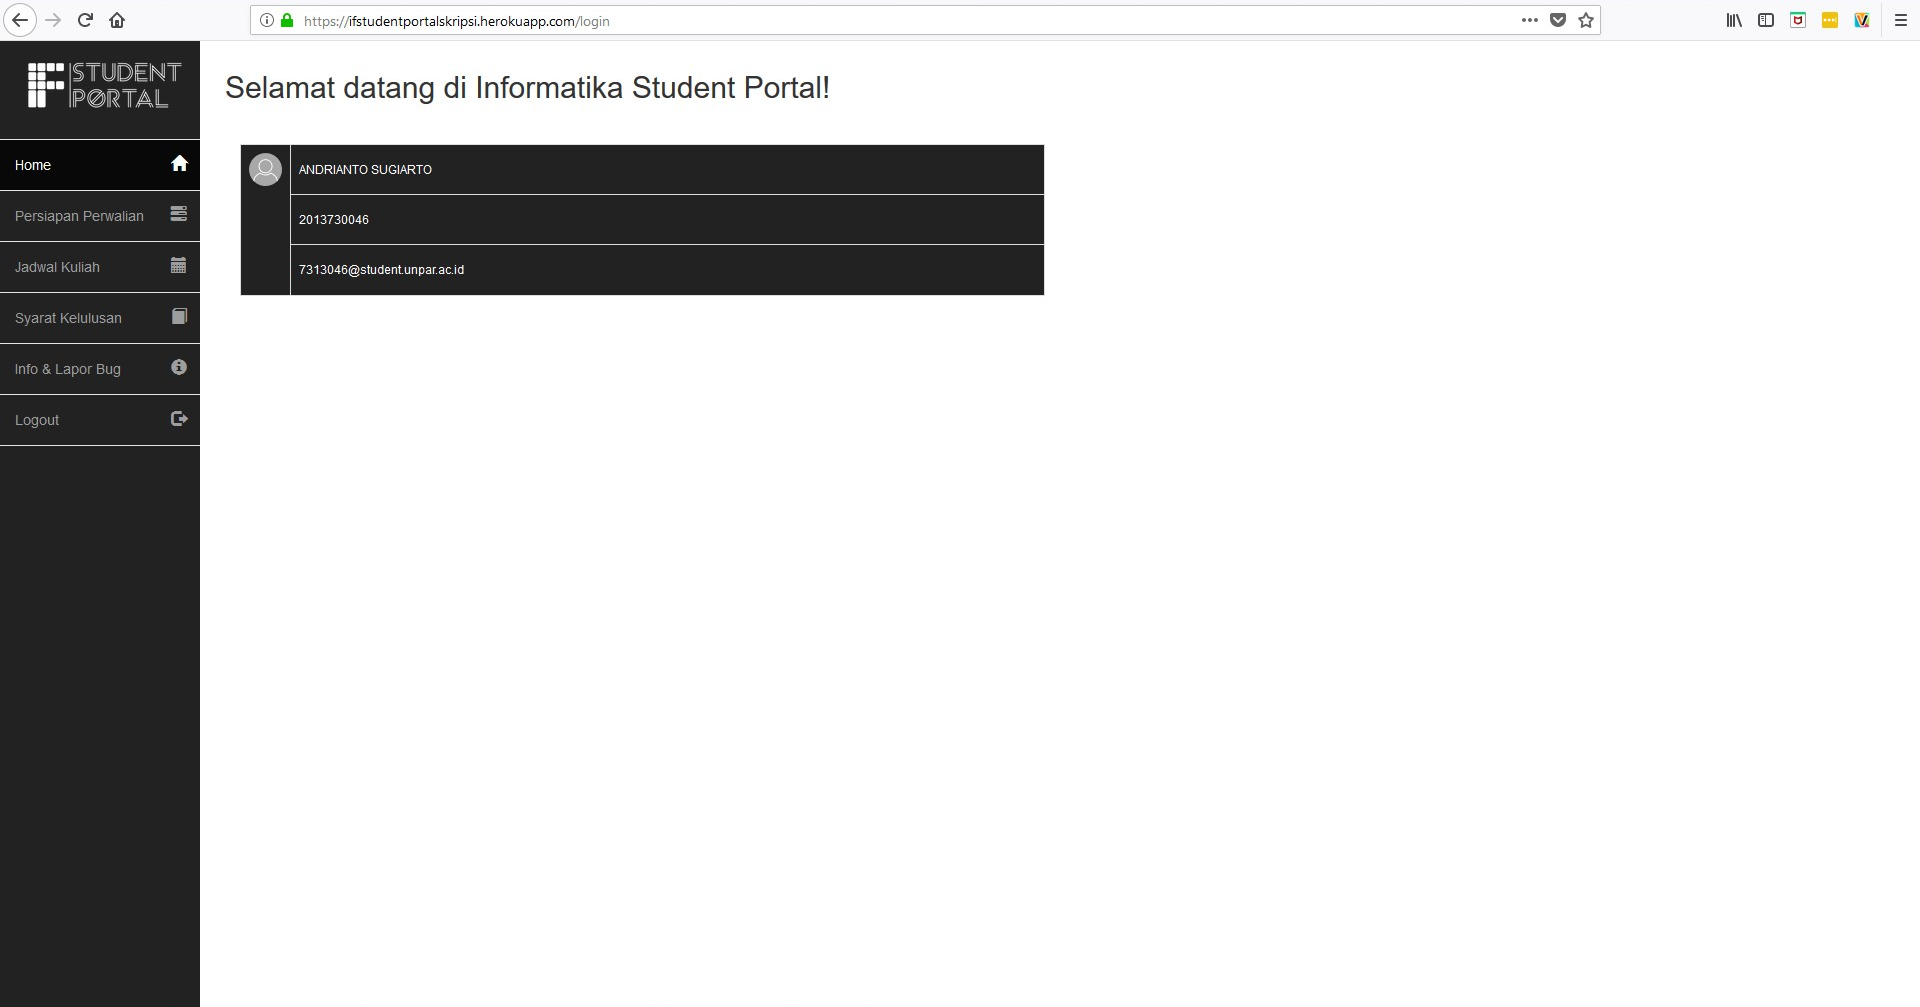
\includegraphics[scale=0.34]{Gambar/halaman_home}
						\caption{Halaman \textit{Home}} 
						\label{fig:5_halaman_utama}
					\end{figure}
						
				\item\textbf{Halaman Persiapan Perwalian}\\
				Halaman ini menampilkan data akademik dan tabel prasyarat mata kuliah. Pengguna dapat mengklik kode mata kuliah, kemudian akan diarahkan ke kode sumber aturan prasyarat mata kuliah tersebut. Tangkapan layar dari halaman prasyarat mata kuliah dapat dilihat pada Gambar \ref{fig:5_halaman_persiapan_perwalian}.
					\begin{figure}[H]
						\centering
						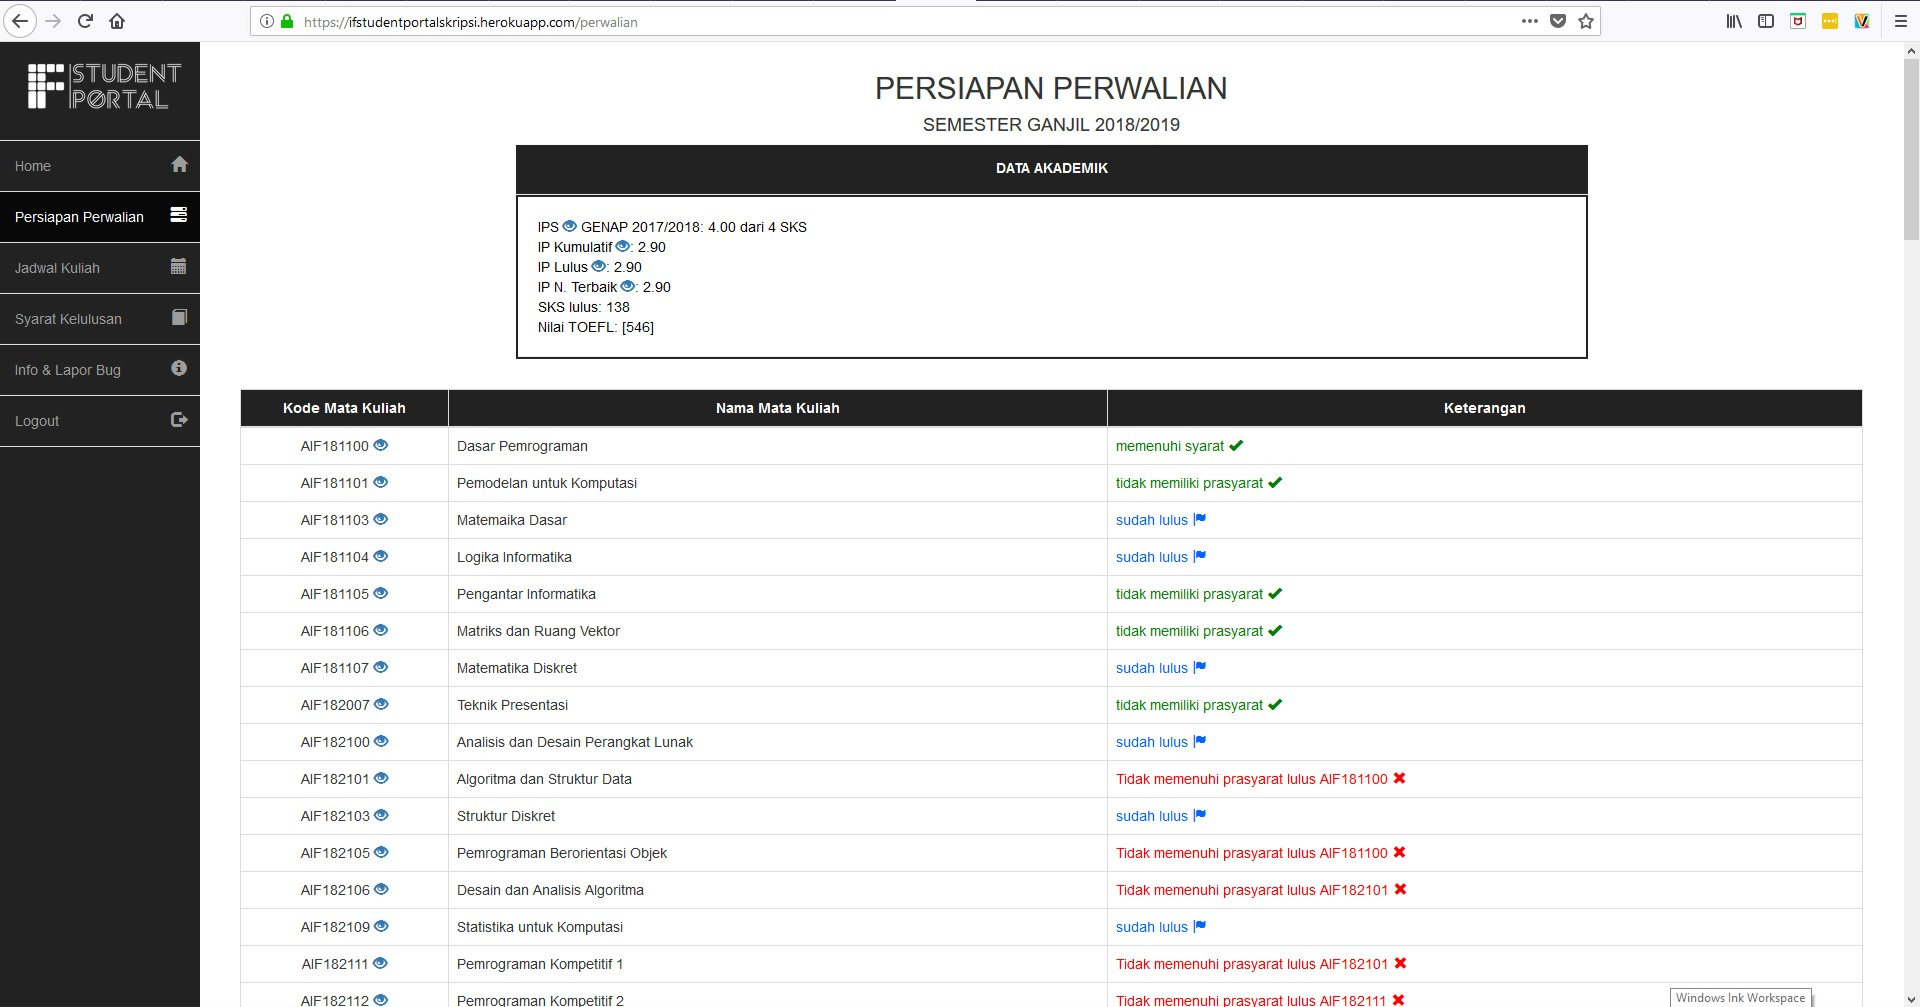
\includegraphics[scale=0.34]{Gambar/halaman_persiapan_perwalian}
						\caption{Halaman Persiapan Perwalian} 
						\label{fig:5_halaman_persiapan_perwalian}
					\end{figure}

				\item\textbf{Halaman Jadwal Kuliah}\\
				Halaman ini menampilkan jadwal kuliah yang tersusun dan terurut berdasarkan hari. Tangkapan layar dari halaman jadwal kuliah dapat dilihat pada Gambar \ref{fig:5_halaman_jadwal}. Jika kode mata kuliah diklik, akan muncul \textit{popup} seperti pada Gambar \ref{fig:5_halaman_jadwal_rinci} yang berisi rincian dari jadwal kuliah tersebut.
				\begin{figure}[H]
						\centering
						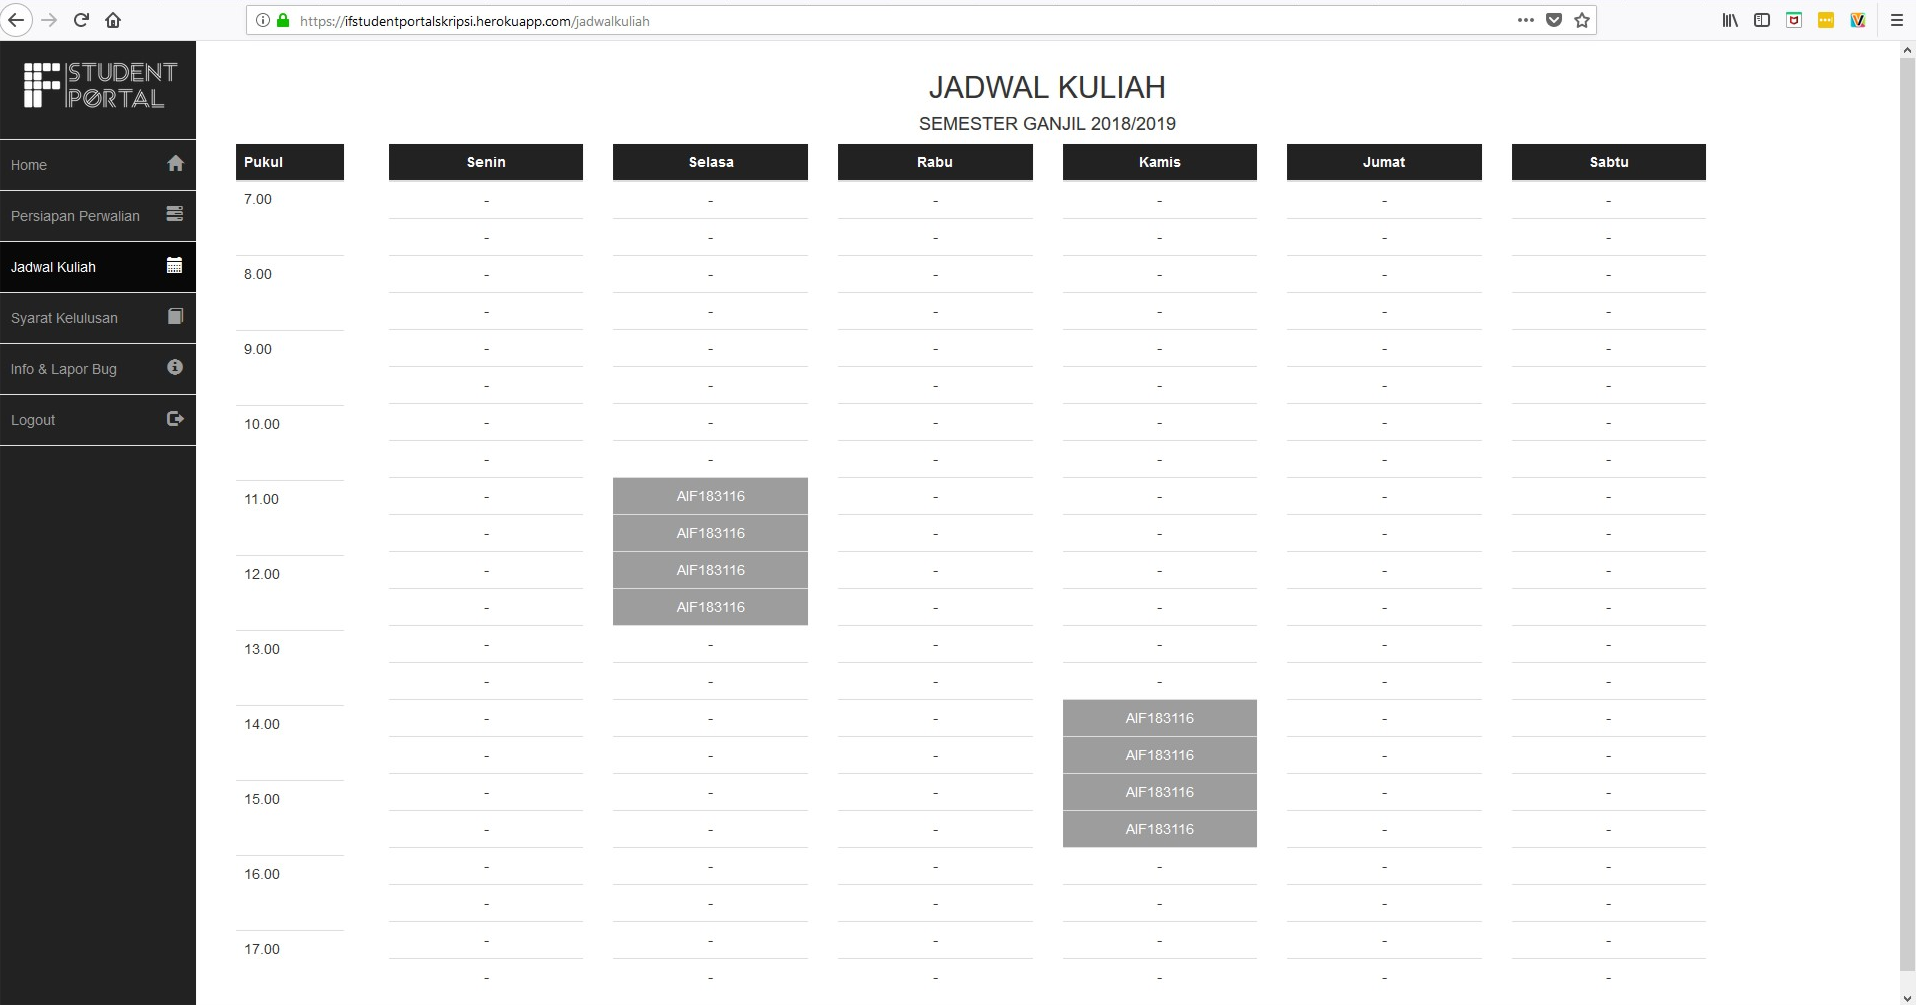
\includegraphics[scale=0.34]{Gambar/halaman_jadwal}
						\caption{Halaman Jadwal Kuliah} 
						\label{fig:5_halaman_jadwal}
					\end{figure}
					
					\begin{figure}[H]
						\centering
						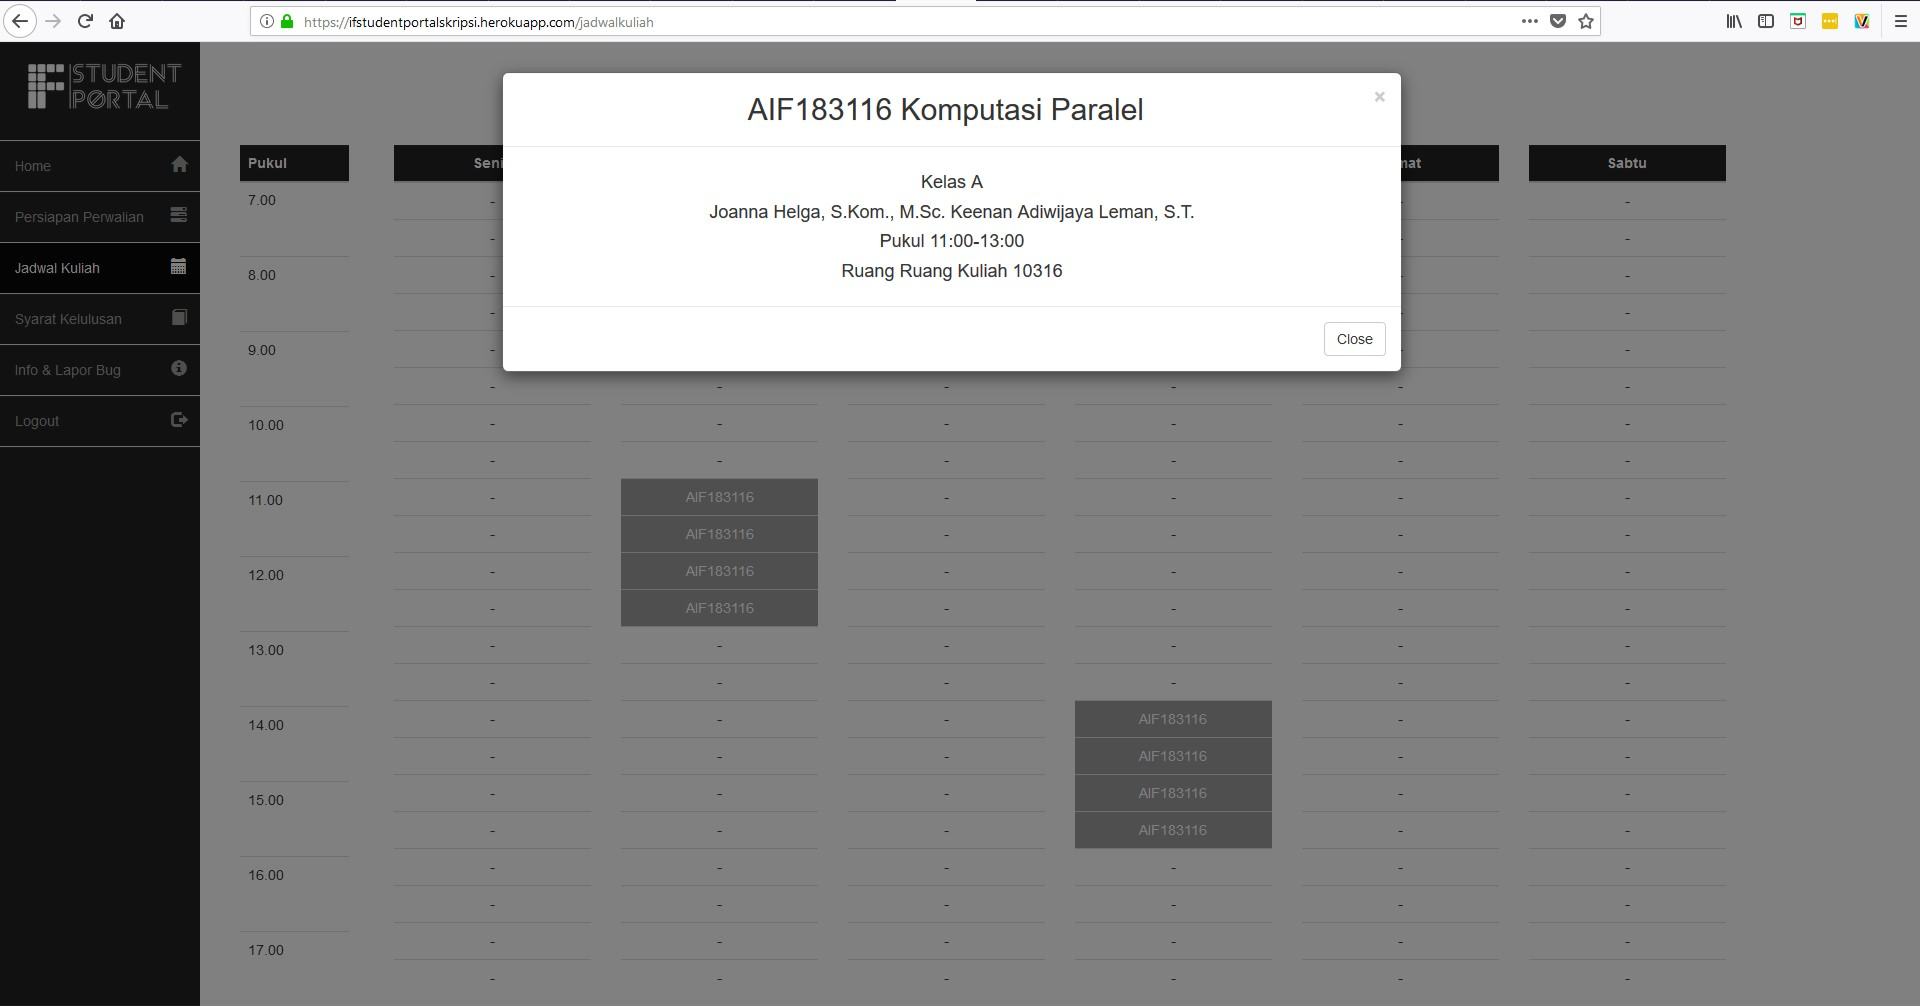
\includegraphics[scale=0.34]{Gambar/halaman_jadwal_rinci}
						\caption{Rincian Jadwal Kuliah} 
						\label{fig:5_halaman_jadwal_rinci}
					\end{figure}
					
				\item\textbf{Halaman Syarat Kelulusan}\\
				Halaman ini menampilkan syarat kelulusan dari Program Studi Teknik Informatika yang belum dipenuhi oleh mahasiswa. Tangkapan layar dari halaman data akademik dapat dilihat pada Gambar \ref{fig:5_halaman_syarat_kelulusan}.
				\begin{figure}[H]
						\centering
						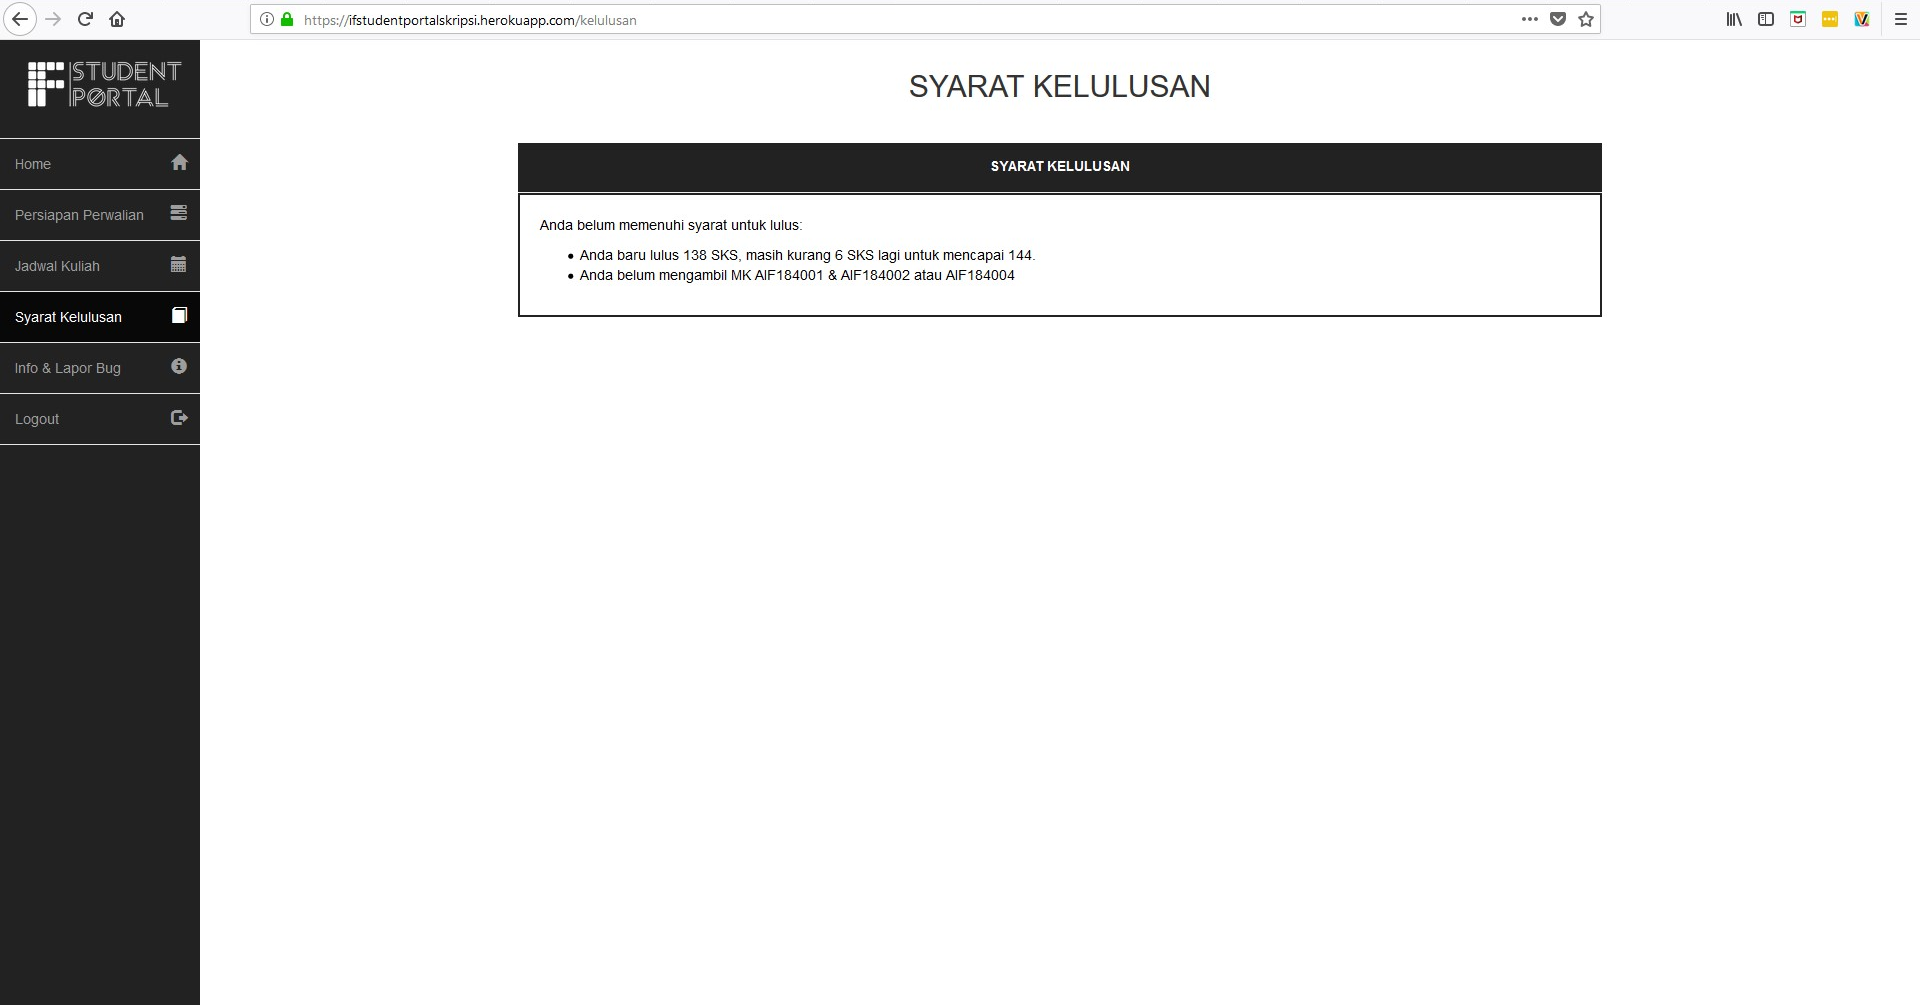
\includegraphics[scale=0.34]{Gambar/halaman_syarat_kelulusan}
						\caption{Halaman Syarat Kelulusan} 
						\label{fig:5_halaman_syarat_kelulusan}
					\end{figure}
		\end{enumerate}
		
\section{Pengujian}

\subsection{Pengujian Fungsional}
\label{subsec:fungsional}

Pengujian fungsional dilakukan untuk mengetahui kesesuaian reaksi perangkat lunak dengan reaksi yang diharapkan berdasarkan aksi pengguna terhadap perangkat lunak. Pengujian dilakukan pada \textit{cloud platform} dan Windows dengan hasil yang sama.

			\begin{table}[H]
			\centering
			\caption{Tabel Pengujian Fungsional}
				\begin{tabular}{|p{0.25cm}| p{3.5cm}| p{7cm}| p{2.5cm}|} \hline
				No.	&	Aksi Pengguna	&	Reaksi yang diharapkan	&	Reaksi Perangkat Lunak \\ \hline
				1.	&	Pengguna menjalankan aplikasi	&	Halaman \textit{login} akan ditampilkan	&	sesuai	\\ \hline
				2.	&	Pengguna memasukkan \textit{email} dan \textit{password}	&	Jika \textit{email} dan \textit{password}	sesuai, pengguna akan diarahkan ke halaman utama. & sesuai\\ \hline
				3.	&	Pengguna memilih menu ``Perwalian'' &	Jika pengguna belum memiliki riwayat nilai(masih menempuh semester 1), akan ditampilkan pesan ``DATA AKADEMIK BELUM TERSEDIA'' dan ``PRASYARAT BELUM TERSEDIA''	&	sesuai	\\ \hline
					&	&	Jika pengguna sudah memiliki riwayat nilai	akan ditampilkan tabel prasyarat mata kuliah beserta status pengambilannya dan ringkasan data akademik mahasiswa berupa IPS semester terakhir, IPK, IP Lulus, IP N. Terbaik, SKS Lulus, dan nilai TOEFL &	sesuai	\\ \hline
				4.	&	Pengguna memilih menu ``Jadwal Kuliah'' &	Jika pengguna belum melakukan FRS, cuti studi, atau jadwal kuliah pengguna belum tersedia, akan ditampilkan pesan ``JADWAL KULIAH BELUM TERSEDIA''	&	sesuai	\\ \hline
					&	&	Jika jadwal kuliah pengguna sudah tersedia, akan ditampilkan jadwal kuliah dalam bentuk kalendar yang sudah diurutkan berdasarkan hari &	sesuai	\\ \hline
				5.	&	Pengguna memilih menu ``Syarat Kelulusan'' &	Jika pengguna belum memiliki riwayat nilai(masih menempuh semester 1), akan ditampilkan pesan ``DATA AKADEMIK BELUM TERSEDIA'' &	sesuai	\\ \hline
					&	&	Jika pengguna sudah memiliki riwayat nilai, akan ditampilkan syarat kelulusan yang belum dipenuhi dari mahasiswa &	sesuai	\\ \hline
				6.	&	Pengguna memilih tombol \textit{logout}	&	Pengguna akan diarahkan kembali ke halaman \textit{login} &	sesuai	\\ \hline
				7.	& Dua pengguna menggunakan aplikasi secara bersamaan	&	Pengguna dapat menggunakan aplikasi dengan akun yang sesuai &	sesuai	\\ \hline
				\end{tabular}
				\label{table:hasilFungsional}
			\end{table}
			
\subsection{Pengujian Eksperimental}
Pengujian eksperimental dilakukan terhadap mahasiswa angkata 2013 sampai 2017. Dari setiap angkatan, diambil satu orang untuk melakukan pengujian. Setiap responden diminta untuk melakukan \textit{login} kemudian melihat dari setiap halaman pada Student Portal dan memastikan apakah data tersebut sesuai dengan data sebenarnya.

Hasil pengujian eksperimental lainnya dirangkum sebagai berikut:
\begin{itemize}
	\item Angkatan 2013
	Saat melakukan pemeriksaan syarat kelulasan, terdapat mahasiswa dengan syarat ``Anda belum mengambil salah satu dari MK Proyek AIF183106 atau AIF183308 \& AIF184303''. Hal ini disebabkan perbedaan kode mata kuliah ``Proyek Sistem Infomasi 2'' dengan \cite{dokumenkurikulum2018}. Pada \cite{dokumenkurikulum2018} dituliskan hasil transisi untuk mata kuliah ``Proyek Sistem Infomasi 2'' adalah ``AIF184303'', sedangkan pada StudentPortal adalah ``AIF134405''. Hal tersebut sudah ditangani dengan menambahkan kode mata kuliah ``AIF134405'' pada pengecekan mata kuliah proyek. Hasil pengujian eksperimental mahasiswa angkatan 2013 sesuai dengan hasil yang diharapkan.
	\item Angkatan 2014
	
	\item Angkatan 2015
	Hasil pengujian eksperimental mahasiswa angkatan 2015 sesuai dengan hasil yang diharapkan.
	\item Angkatan 2016
	
	\item Angkatan 2017
	
	\item Angkatan 2018
	
\end{itemize}